\chapter{Literature Review}\label{ch:literature-review}


\section{Introduction}\label{sec:introduction}

This chapter reviews existing literature across three interconnected areas: \textbf{impact measurement and management (IMM)}, \textbf{public sector innovation (PSI)}, and the application of \textbf{artificial intelligence (AI)} in these domains.
The goal is to establish a conceptual foundation for AI-supported, values-driven impact evaluation in public innovation ecosystems.

\section{Impact Measurement and Management (IMM)}\label{sec:impact-measurement-and-management-imm}

The measurement of impact, especially within social or public contexts, has evolved significantly in recent years.

\begin{figure}[H]
    \centering
    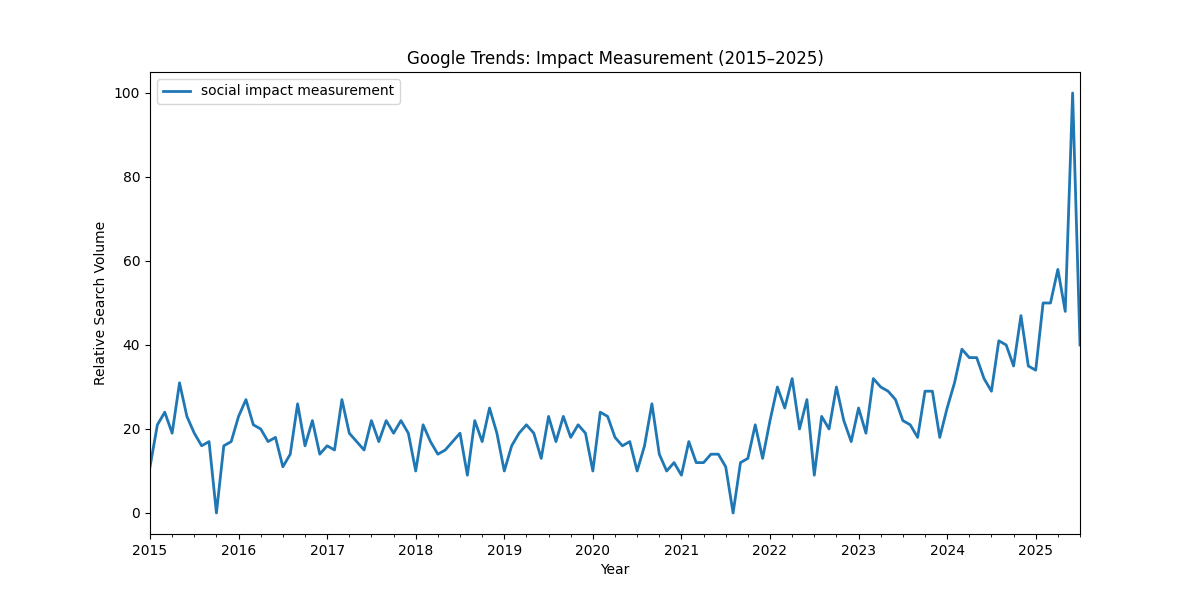
\includegraphics[width = 0.8\textwidth]{../fig/google_trend_impact}
    \caption{Google trend of "impact measurement"}
    \label{fig:trend_impact}
\end{figure}

Scholars such as \textcite{ebrahim2014measuring} emphasize the need to align measurement approaches with a theory of change and organizational strategy.
They argue that organizations often struggle to balance accountability and learning, especially when the impact is diffuse or long-term.


\textcite{nicholls2012measuring} highlight the tensions between standardized, quantitative measurement systems and the contextual, qualitative nature of many social interventions.
Their work in the field of social entrepreneurship has helped formalize a typology of impact logic models, demonstrating that one-size-fits-all approaches rarely succeed.

In the German context, actors like Phineo and UnternehmerTUM have offered practical IMM frameworks tailored to social enterprises and innovation labs.
These models combine stakeholder mapping, output-outcome mapping, and logic modelling to foster clarity in how public interventions are expected to generate value.

\section{Public Sector Innovation and Value Creation}\label{sec:public-sector-innovation-and-value-creation}

Public sector innovation requires institutions not only to introduce new tools or practices, but also to foster new forms of legitimacy, collaboration, and accountability~\parencite{sun2019algorithmic}.
The OECD has extensively documented the challenges and opportunities that come with innovation in government, including a growing emphasis on public value creation, citizen co-production, and agile experimentation~\parencite{oecd2020publicsector}.

\textcite{wirtz2020public} provide a conceptual model for the digital transformation of public services, noting that data-driven approaches can both enhance and erode trust depending on their transparency, inclusiveness, and perceived fairness.

The concept of \textbf{public value}—first developed by Moore (1995) and later expanded in various governance frameworks—has become a central reference point for assessing the outcomes of innovation.
This aligns with the mission of the Public Value Hub and serves as a guiding principle in Project Athena.

\section{Artificial Intelligence in Evaluation and Decision-Making}\label{sec:artificial-intelligence-in-evaluation-and-decision-making}

Artificial intelligence has seen increased use in public governance contexts—from algorithmic decision-making to NLP-based policy analysis.
\textcite{devlin2018bert} introduced BERT, a transformer-based model for language understanding that has since become foundational for text classification, topic modeling, and semantic similarity tasks—tools that can be applied in impact evaluation scenarios.
\textcite{sun2019algorithmic} caution that AI must be embedded in deliberative and adaptive governance systems to ensure that its use enhances, rather than replaces, human judgment.
Recent work by \textcite{brown2020algorithmic} explores how algorithmic systems can improve accountability by automating monitoring, but also warns of risks such as value misalignment, opacity, and exclusion.
Rather than automating decision-making, Project Athena employs AI to augment human insight —especially in understanding complex, qualitative narratives.

\section{Synthesis and Gaps}\label{sec:synthesis-and-gaps}

Impact Measurement and Management (IMM), public innovation, and AI-supported decision-making provide complementary approaches to address complex societal challenges in the public sector.
However, an integrated framework unifying these domains remains underdeveloped.
Current IMM approaches, designed to evaluate social, environmental, and economic impacts, often rely on structured metrics, limiting their ability to process unstructured data such as stakeholder feedback or social media sentiment~\cite{epstein_yuthas_2014}.
Similarly, AI applications in public sector evaluation prioritize technical efficiency over social complexity and normative commitments, such as transparency and equity, central to public value creation~\cite{moore_1995,benington_moore_2011}.
This thesis addresses these gaps by proposing a use case where AI augments human interpretation, grounded in stakeholder input, aligned with public value frameworks, and informed by trusted German intermediaries.

IMM offers a systematic method to assess impacts of public initiatives, such as digital inclusion or sustainability programs~\cite{epstein_yuthas_2014}.
However, its focus on quantitative indicators often overlooks qualitative, unstructured data critical for capturing diverse stakeholder perspectives~\cite{fraunhofer_2023}.
For instance, German intermediaries like the Fraunhofer Institute apply IMM in smart city projects but rarely incorporate qualitative social inputs~\cite{fraunhofer_2023}.
Public innovation, emphasizing co-creation and stakeholder engagement, ensures legitimacy and alignment with public values~\cite{moore_1995,benington_moore_2011}.
Initiatives like CityLAB Berlin and GovTech Campus Deutschland exemplify this through participatory design, yet they underutilize AI to scale stakeholder input analysis~\cite{citylab_2024}.

AI, particularly natural language processing (NLP), can bridge these gaps by analyzing unstructured data, such as public consultation transcripts or social media posts~\cite{oecd_2023}.
However, public sector AI often neglects social complexity and normative commitments, risking biases and reduced trust~\cite{eu_2024}.
The proposed framework integrates IMM’s impact-focused evaluation, public innovation’s stakeholder-driven legitimacy, and AI’s analytical capabilities.
A use case illustrates this: a Hamburg municipality aims to measure the impact of a digital inclusion program for equitable broadband access by 2030.
AI-driven NLP, using German BERT~\cite{huggingface_2023}, analyzes unstructured data from public forums to identify barriers (e.g., affordability).
Stakeholders, engaged via GovTech Campus Deutschland, validate these insights to refine impact metrics and co-design interventions (e.g., training programs).
Outcomes are evaluated using Moore’s public value framework~\cite{moore_1995}, balancing efficiency, impact, and legitimacy.
Informed by Fraunhofer’s IMM expertise and DIN’s AI standards~\cite{din_2023}, this framework aligns with Germany’s Digital Strategy 2025~\cite{bmwi_2022}, offering a scalable model for impact-driven public innovation.

This framework bridges IMM’s technical limitations and AI’s normative shortcomings, contributing to inclusive, transparent, and effective public sector decision-making.

\section{Conclusion and Research Direction}\label{sec:conclusion-and-research-direction}


This thesis proposes a values-aligned, AI-assisted approach to public sector impact measurement—grounded in stakeholder experience, practical frameworks, and intelligent tools that make sense of complexity without losing context.
The next chapter outlines the methodology used to develop and test this integrated approach.
